
\begin{SCfigure}
	\centering
	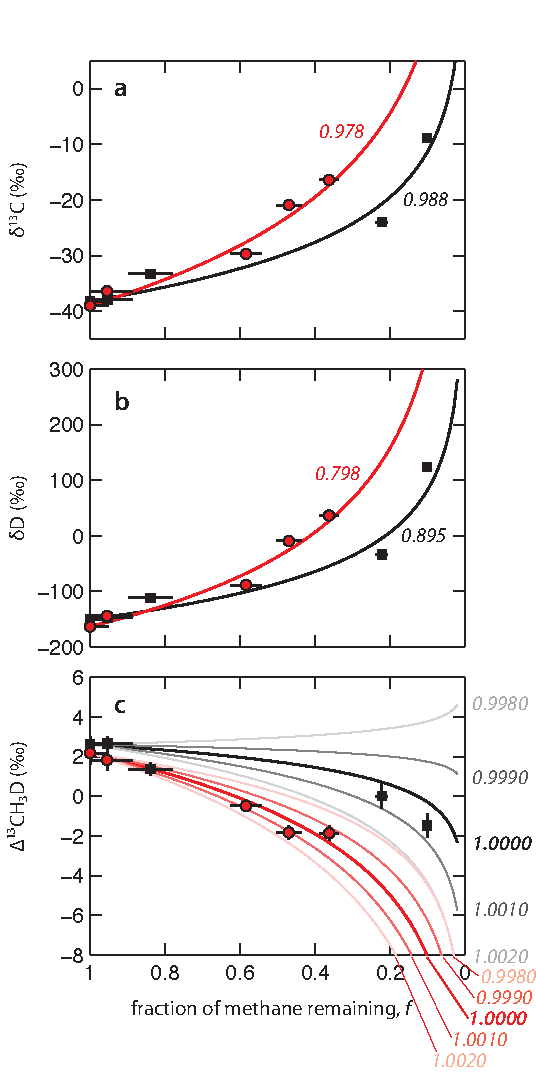
\includegraphics[width=0.5\textwidth]{figures/Fig4.1}
	\caption[Measured and modeled δ\textsuperscript{13}C, δD, and Δ\textsuperscript{13}CH\textsubscript{3}D values in batch cultures]{Measured and modeled changes in \textbf{(a)}
		δ\textsuperscript{13}C, \textbf{(b)} δD, and \textbf{(c)}
		Δ\textsuperscript{13}CH\textsubscript{3}D of residual methane as a
		function of \emph{f}, the fraction of initial methane remaining. Data
		points from the 30 and 37~°C experiments (\autoref{tab:4:1}) are shown with black
		and red symbols, respectively. Horizontal error bars represent
		propagated ±1$\sigma$ uncertainties from GC measurements, and vertical error
		bars represent 95\% confidence intervals from isotopologue ratio
		analyses. Solid lines represent the modeled values (from \mrefs[]{Eqns.}{eqn:4:13}, \ref{eqn:4:16},
		and \ref{eqn:4:20}) based on the calculated weighted-average carbon- and
		hydrogen-isotope fractionation factors for each set of experiments as
		listed in \autoref{tab:4:1}. Labels in \emph{italics} represent
		\textsuperscript{13}$\alpha$, \textsuperscript{D}$\alpha$, \& $\gamma$, respectively, in
		panels (a), (b), \& (c). Panel (c) shows model results calculated
		assuming different values of $\gamma$ varying between 0.9980 and 1.0020.}
	\label{fig:4:1}
\end{SCfigure}